\documentclass{article}
\usepackage{relsize}
\usepackage{array}
\usepackage{tabularx}
\usepackage{imakeidx}
\usepackage{float}
\usepackage[T1]{fontenc}
\usepackage{graphics}
\usepackage{xcolor}
\usepackage{etoolbox}
\usepackage{graphicx}
\usepackage{rotating}
\usepackage{float}

\colorlet{darkGreen}{green!40!black}

\newcommand{\databaseTable}[2]{
	\begin{table}[H]
		\centering
		\renewcommand{\arraystretch}{1.5}
		\begin{tabularx}{\textwidth}{|c|c|c|c|>{\centering\arraybackslash}X|}
			\hline
			\textbf{Nombre del campo} & \textbf{Tipo de dato} & \textbf{PK} & \textbf{FK} & \textbf{Descripción} \\
			\hline
			#1                                                                                                   \\
			\hline
		\end{tabularx}
		\caption{#2}
	\end{table}
}

\newcommand{\entidadBullets}[3]
{
	\subsubsection{#1}
	\begin{sloppy}
		\begin{itemize}
			\item Especificaciones:
			      #2
			\item Consideraciones:
			      #3
		\end{itemize}
	\end{sloppy}
}

\newcommand{\modeloRelacionalItem}[2]
{
	\item \textcolor{darkGreen}{#1}(#2)
}

\newcommand{\blue}[1]{\textcolor{blue}{#1}}

\newcommand{\green}[1]{\textcolor{darkGreen}{#1}}
\renewcommand{\contentsname}{Contenidos}
\makeindex[columns=3, title=Alphabetical Index, intoc]
\begin{document}
\begin{titlepage}
	\centering
	\bfseries\LARGE{Universidad de Ingeniería y Tecnología} \par
	\vspace{1cm}
	\Large\scshape{Facultad de Computación} \par
	\vspace{2cm}
	\scshape\Huge{ERP PARA INSTITUCIONES DE EDUCACIÓN PRIMARIA Y SECUNDARIA} \par
	\vspace{2cm}
	\scshape\Large{Hito 2} \par
	\vfill
	\Large{Autores:} \par
	\Large Escobar Núñez, Alejandro Ismael \\
	Silva Rios, Alessandra Valeria \\
	Galvez Pacori, José Guillermo \par
	\vfill
	\Large Profesor: \par
	\Large Rios Ojeda, Brenner Humberto \par
	\vfill
	\Large{Julio, 2024} \par
\end{titlepage}
\tableofcontents{}
\newpage{}
\section{Requisitos}
\subsection{Introducción}
En el mundo actual, las instituciones educativas son más que solo lugares de aprendizaje. Son microcosmos complejos que requieren una gestión eficiente y coordinada de una multitud de operaciones administrativas, académicas y operativas. Sin embargo, a medida que estas instituciones crecen y se vuelven más complejas, la gestión eficiente de estas operaciones se convierte en un desafío cada vez mayor.

Este desafío se ve agravado por la falta de sistemas de gestión eficientes que puedan manejar la creciente complejidad de las operaciones de las instituciones educativas. La falta de eficiencia y coordinación en la gestión de estas operaciones puede llevar a una serie de problemas, desde la mala gestión de los recursos hasta la insatisfacción de los estudiantes y los padres.

En este informe, abordaremos un problema específico que enfrentan muchas instituciones educativas: la falta de eficiencia y coordinación en la gestión administrativa, académica y operativa. Este problema no solo afecta la calidad de la educación que se ofrece, sino que también puede tener un impacto negativo en la reputación de la institución.

El objetivo de este proyecto es desarrollar una base de datos que pueda ayudar a abordar este problema. Con esto en mente, esperamos que este informe sirva como un punto de partida para entender la magnitud del problema y la necesidad de una solución efectiva. A medida que avanzamos desde una visión general de las instituciones educativas hasta un enfoque más específico en la necesidad de automatización, esperamos proporcionar una visión clara y detallada del problema que se resolverá.
\subsection{Descripción general del problema} (Ismael)
\subsection{Necesidad y usos de la base de datos} (Ismael)
\subsection{¿Cómo resuelve el problema hoy?} (Alessandra)
\subsubsection{¿Cómo se almacenan y procesan los datos?}
\subsubsection{Flujo de datos}
\subsection{Descripción detallada del sistema} (Alessandra)
\subsubsection{Objetos de información actuales}
\subsubsection{Características y funcionalidades esperadas}
\subsubsection{Tipos de usuarios existentes o necesarios}
\subsubsection{Tipo de consulta y actualizaciones} (Ismael)
\subsubsection{Tamaño estimado de la base de datos} (Ismael)
\subsection{Objetivos del proyectos} (Alessandra)
\subsection{Referencias del proyecto} (Alessandra)
\subsection{Eventualidades} (Ismael)
\subsubsection{Problemas que pudieran encontrarse en el proyecto}
\subsubsection{Límites y alcances del proyecto}
\section{Modelo Entidad-Relación}
\subsection{Reglas semánticas}
\begin{itemize}
	\item Una institución tiene descripción, banner, nombre, fue fundado en cierta fecha y por alguien, y tiene RUC como identificador.
	\item Una institución tiene al menos una sede, y en ella trabajan colaboradores y se dictan clases.
	\item Una persona tiene nombres, apellidos, fecha de nacimiento, sexo, email y es identificada por su DNI.
	\item Un alumno es una persona, puede ser matriculado por solo un apoderado y estudia en un solo salón.
	\item Un apoderado es una persona, tiene número de celular y puede matricular a uno o más alumnos.
	\item Un colaborador es una persona, tiene sueldo por hora, cci, numero de celular, horas semanales de trabajo y necesitamos saber si está activo o no.
	\item Un profesor es un colaborador y trabaja en una o más sedes enseñando uno o más cursos en uno o más grados en cierto periodo académico.
	\item Un secretario es un colaborador y trabaja en una sola sede.
	\item Un director es un colaborador y dirige una sola sede.
	\item Un consejero es un colaborador y trabaja en una sola sede.
	\item Un tutor es un colaborador, trabaja en una sola sede y se le asigna vigilar un solo salón.
	\item Una sede tiene un id como identificador, una dirección y sus respectivas coordenadas, además de la fecha de su construcción, es dirigida por un solo director y en ella trabajan, uno o más consejeros, uno o más secretarios, uno o más tutores y uno o más profesores, y tiene uno o más salones.
	\item Un salón tiene un nombre de sección como llave parcial, cuenta con un número para el aforo, además, pertenece a una sola sede, es vigilado por un tutor, en él estudian muchos alumnos y en él se dictan clases de un solo grado.
	\item Un grado está identificado por un id, tiene un nombre, las clases de un grado son dictadas en uno o más salones por un profesor en cierto periodo académico y este contiene muchos cursos.
	\item Un curso está identificado por un id, posee un nombre, está dictado por un profesor y está contenido en uno o más grados.
	\item Una matrícula es realizada en cierto año por un apoderado al darle los datos de un alumno a un secretario para que lo registre en un grado y una sede.
\end{itemize}
\begin{landscape}
	\subsection{Modelo Entidad-Relación}
	\begin{figure}[H]
		\centering
		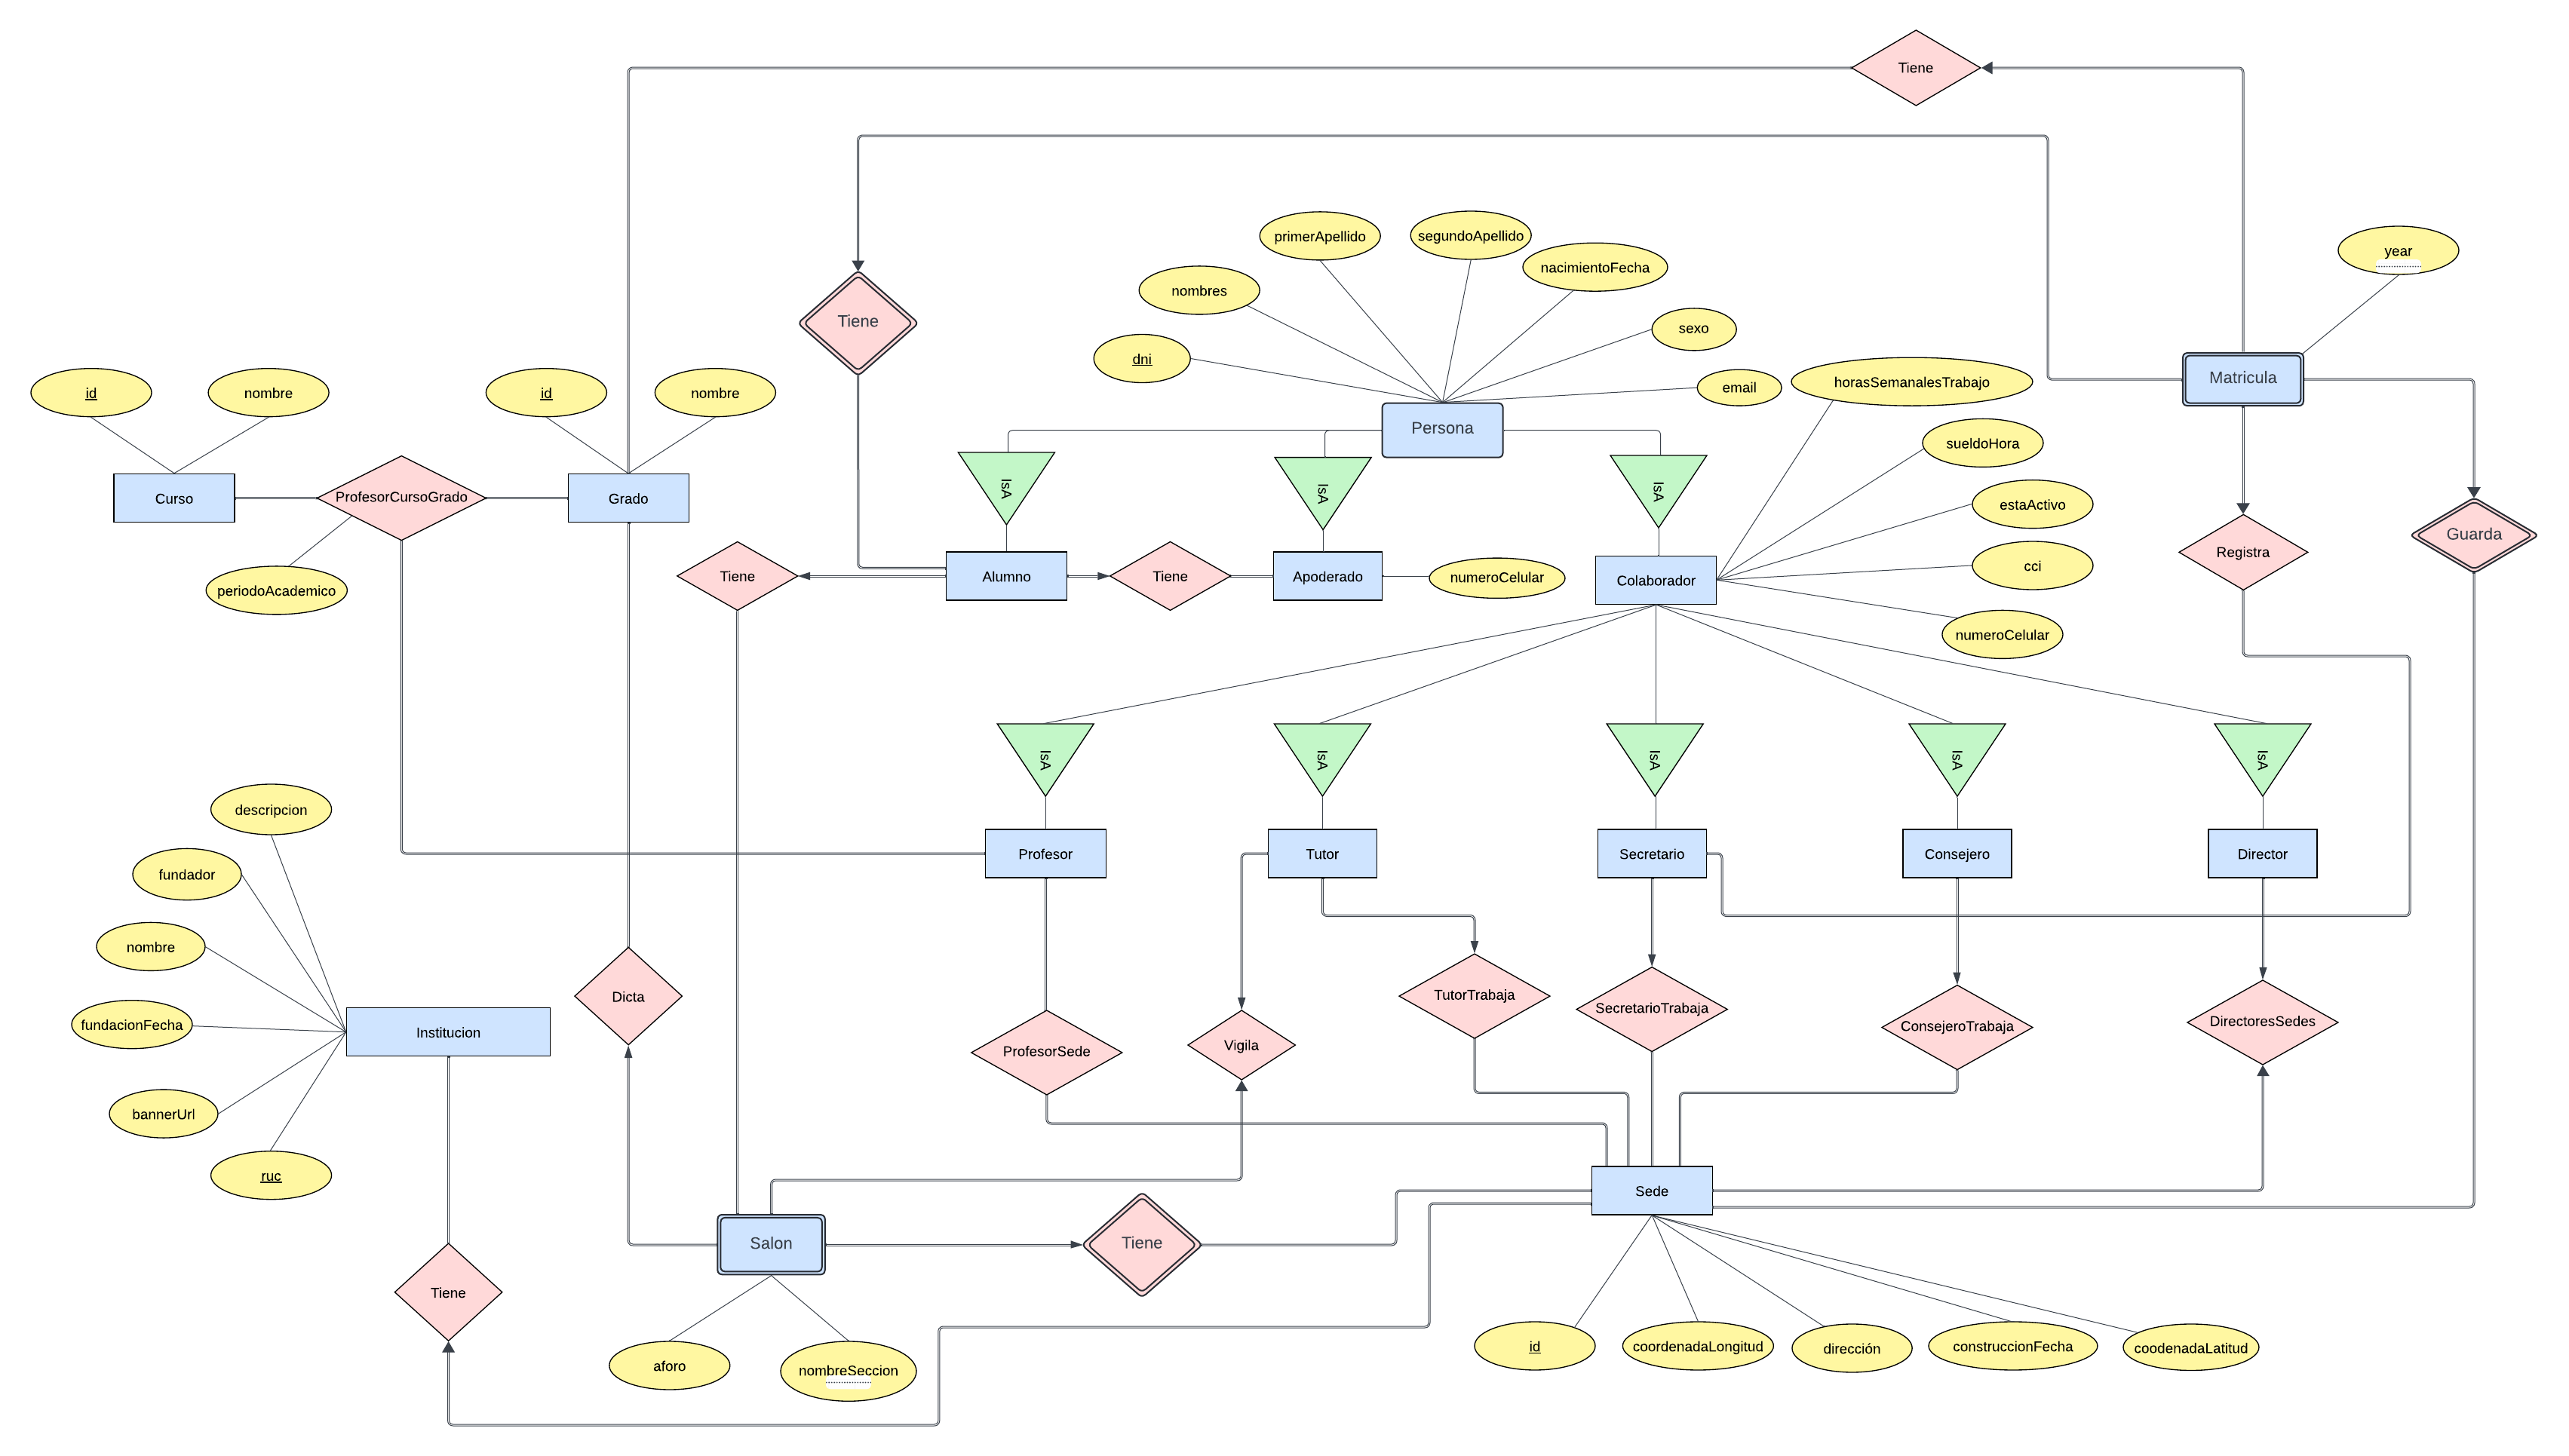
\includegraphics[width=\textheight, height=\textheight, keepaspectratio]{figures/modeloer-latest.png}
		\caption{Modelo Entidad-Relación}
		\label{fig:my_label}
	\end{figure}
\end{landscape}
\newpage
\subsection{Especificaciones y consideraciones sobre el modelo}
\entidadBullets{Entidad Institucion}{Almacena la información más importante de cada institución: descripción, banner, nombre, fecha de fundación, fundador y el RUC como llave primaria.}{El RUC es seleccionado como la llave primaria ya que es un identificador único y oficial para cada institución. Esto facilita la gestión administrativa y legal de la información de la institución. Esta entidad no posee relaciones con ninguna otra entidad, ya que solo almacenerá una tupla la cual tendrá la información antes descrita.}
\entidadBullets{Entidad Persona}{Almacena la información más importante de cada individuo, incluyendo DNI (como llave primaria), nombres, apellidos, fecha de nacimiento, sexo y email.}{El DNI es usado como llave primaria, proporcionando un medio único y eficiente para identificar a cada persona. Esta entidad actúa como una superclase que hereda a las subclases Alumno, Apoderado y Colaborador, permitiendo solapamiento y cobertura total.}
\entidadBullets{Entidad Alumno}{Subclase de Persona. Está vinculado a un único salón y es matriculado por un solo apoderado.}{Hereda el DNI de Persona como llave primaria. La relación exclusiva con un apoderado y un salón justifica el mantenimiento de estas conexiones a través de claves foráneas, lo cual asegura integridad referencial y facilita consultas relacionales.}
\entidadBullets{Entidad Apoderado}{Subclase de Persona. Posee un número de celular adicional y puede matricular a uno o más alumnos.}{Utiliza el DNI de Persona como llave primaria. La capacidad de vincularse con múltiples alumnos refuerza su rol en el proceso educativo y administrativo, y la integridad referencial se mantiene a través de relaciones definidas en la base de datos.}
\entidadBullets{Entidad Colaborador}{Subclase de Persona. Incluye sueldo por hora, CCI, número de celular, horas semanales de trabajo y un atributo para saber si está activo o no.}{Continúa usando el DNI como llave primaria. Actúa como superclase para Profesor, Secretario, Director, Consejero, y Tutor, facilitando la implementación de políticas de empleo y administración dentro del colegio.}
\entidadBullets{Entidad Profesor}{Subclase de Colaborador. Puede enseñar en una o más sedes.}{Mantiene el DNI como llave primaria. La flexibilidad de enseñar en múltiples sedes es gestionada mediante una relación muchos a muchos con Sede, lo cual permite una programación eficiente.}
\entidadBullets{Entidad Secretario}{Secretario es una subclase de Colaborador y trabaja en una sola sede.}{El DNI es la llave primaria.Establece una relación muchos a uno con Sede la cual es justificada a través de una clave foránea, lo que garantiza que cada sede tenga un único secretario asociado.}
\entidadBullets{Entidad Director}{Director es una subclase de Colaborador y dirige una sola sede.}{El DNI es la llave primaria y sedeId como llave foránea. La exclusividad de la relación uno a uno con Sede asegura un manejo claro de responsabilidades administrativas.}
\entidadBullets{Entidad Consejero}{Consejero es una subclase de Colaborador y trabaja en una sede.}{Utiliza el DNI como llave primaria. La relación muchos a uno con Sede facilita la asignación de responsabilidades y roles dentro del colegio y realiza la conexión a través de una llave foránea.}
\entidadBullets{Entidad Tutor}{Tutor es una subclase de Colaborador, trabaja en una sede y se le asigna un salón.}{El DNI como llave primaria, nombreSeccion y sedeId como llaves foráneas, además su relación específica con un salón ayuda a mantener un control efectivo sobre el ambiente educativo.}
\entidadBullets{Entidad Sede}{Sede tiene un identificador único (ID), dirección, coordenadas y fecha de construcción. Está dirigida por un Director.}{El ID como llave primaria y el RUC de la institución como llave foránea.}
\entidadBullets{Entidad Salon}{Salón tiene como identificador nombreSeccion, tiene aforo, pertenece a una sede, en este se dictan clases de un grado y es supervisado por un Tutor.}{Tiene una llave primaria compuesta por los atributos nombreSeccion y sedeId, además de tener a gradoId como llave foránea lo cual permite un manejo detallado de los espacios físicos. Es considerada una entidad débil, ya que no podría existir un salón si es que no existe una sede al igual que no tendría sentido tener un salón sin que ninguna clase de algún grado se realice en él.}
\entidadBullets{Entidad Grado}{Grado está identificado por un ID y tiene un nombre. Contiene varios cursos y se enseña en varios salones.}{El ID como llave primaria facilita la organización de los programas educativos. Se relaciona con Profesor, Curso y Salón para estructurar el currículo.}
\entidadBullets{Entidad Curso}{Curso tiene un ID y un nombre, y está contenido en uno o más grados.}{El ID como llave primaria es adecuado para la gestión curricular. La relación con Grado y Profesor permite múltiples configuraciones pedagógicas.}
\entidadBullets{Entidad Matrícula}{Involucra Alumno, Apoderado, Grado, Sede y es realizada por un Secretario. Usa una clave primaria compuesta de alumnoDni, year, y sedeId.}{La clave primaria compuesta asegura una identificación única de cada registro, facilitando la administración y el seguimiento académico. Es una entidad débil, ya que para existir necesita que un apoderado matricule a un alumno con la ayuda de un secretario en cierto grado en cierta sede.}
\section{Modelo Relacional}
\subsection{Modelo Relacional}
\begin{itemize}
	\modeloRelacionalItem{\textcolor{darkGreen}{InformacionInstitucion}}{\underline{\textcolor{blue}{ruc}}, \textcolor{blue}{descripcion}, \textcolor{blue}{fundador}, \textcolor{blue}{fundacionFecha}, \textcolor{blue}{bannerUrl}, \textcolor{blue}{nombre}}
	\modeloRelacionalItem{\textcolor{darkGreen}{Persona}}{\underline{\textcolor{blue}{dni}}, \textcolor{blue}{nombre}, \textcolor{blue}{primerApellido}, \textcolor{blue}{segundoApellido}, \textcolor{blue}{nacimientoFecha}, \textcolor{blue}{sexo}, \textcolor{blue}{email}}
	\modeloRelacionalItem{\textcolor{darkGreen}{Apoderado}}{\underline{\textcolor{blue}{\textcolor{darkGreen}{Persona}.dni}}, \textcolor{blue}{numeroCelular}}
	\modeloRelacionalItem{\textcolor{darkGreen}{Alumno}}{\underline{\textcolor{blue}{\textcolor{darkGreen}{Persona}.dni}}, \textcolor{blue}{\textcolor{darkGreen}{Salon}.nombreSeccion}, \textcolor{darkGreen}{Grado}.\textcolor{blue}{id}, \textcolor{darkGreen}{Sede}.\textcolor{blue}{id}, \textcolor{darkGreen}{Apoderado}.\textcolor{blue}{dni}}
	\modeloRelacionalItem{\textcolor{darkGreen}{Colaborador}}{\underline{\textcolor{blue}{\textcolor{darkGreen}{Persona}.dni}}, \textcolor{blue}{sueldoMensual}, \textcolor{blue}{cci}, \textcolor{blue}{numeroCelular}, \textcolor{blue}{horasSemanalesTrabajo}}
	\modeloRelacionalItem{\textcolor{darkGreen}{Secretario}}{\underline{\textcolor{blue}{\textcolor{darkGreen}{Colaborador}.dni}}, \textcolor{darkGreen}{Sede}.\textcolor{blue}{id}}
	\modeloRelacionalItem{\textcolor{darkGreen}{Consejero}}{\underline{\textcolor{blue}{\textcolor{darkGreen}{Colaborador}.dni}}, \textcolor{darkGreen}{Sede}.\textcolor{blue}{id}}
	\modeloRelacionalItem{\textcolor{darkGreen}{Tutor}}{\underline{\textcolor{blue}{\textcolor{darkGreen}{Colaborador}.dni}}, \textcolor{darkGreen}{Sede}.\textcolor{blue}{id}}
	\modeloRelacionalItem{\textcolor{darkGreen}{Profesor}}{\underline{\textcolor{blue}{\textcolor{darkGreen}{Colaborador}.dni}}}
	\modeloRelacionalItem{\textcolor{darkGreen}{ProfesorSede}}{\underline{\textcolor{blue}{\textcolor{darkGreen}{Profesor}.dni}}, \textcolor{darkGreen}{Sede}.\textcolor{blue}{id}}
	\modeloRelacionalItem{\textcolor{darkGreen}{Sede}}{\underline{\textcolor{blue}{id}}, \textcolor{blue}{coordenadaLongitud}, \textcolor{blue}{coordenadaLatitud}, \textcolor{blue}{direccion}, \textcolor{blue}{construccionFecha}, \textcolor{darkGreen}{Director}.\textcolor{blue}{dni}}
	\modeloRelacionalItem{\textcolor{darkGreen}{Grado}}{\underline{\textcolor{blue}{id}}, \textcolor{blue}{nombre}}
	\modeloRelacionalItem{\textcolor{darkGreen}{Curso}}{\underline{\textcolor{blue}{id}}, \textcolor{blue}{nombre}}
	\modeloRelacionalItem{\textcolor{darkGreen}{ProfesorCursoGrado}}{\underline{\textcolor{blue}{\textcolor{darkGreen}{Curso}.id}}, \underline{\textcolor{blue}{\textcolor{darkGreen}{Grado}.id}}, \underline{\textcolor{blue}{\textcolor{darkGreen}{Profesor}.dni}}, \textcolor{blue}{periodoAcademico}}
	\modeloRelacionalItem{\textcolor{darkGreen}{Salon}}{\textcolor{blue}{aforo}, \underline{\textcolor{blue}{nombreSeccion}}, \textcolor{darkGreen}{Grado}.\textcolor{blue}{id}, \underline{\textcolor{blue}{\textcolor{darkGreen}{Sede}.id}}, \textcolor{darkGreen}{Tutor}.\textcolor{blue}{dni}}
	\modeloRelacionalItem{\textcolor{darkGreen}{Matricula}}{\underline{\textcolor{blue}{year}}, \underline{\textcolor{blue}{\textcolor{darkGreen}{Alumno}.dni}}, \underline{\textcolor{blue}{\textcolor{darkGreen}{Sede}.id}}, \textcolor{darkGreen}{Grado}.\textcolor{blue}{id}, \textcolor{darkGreen}{Secretario}.\textcolor{blue}{dni}}
\end{itemize}
\subsection{Especificaciones de transformación}
\subsubsection{Entidades}
\begin{itemize}
	\item \textbf{Curso:} Se transforma en la tabla Curso con id como llave primaria. Cada curso tiene un nombre único. No hay dependencia directa con otras tablas a nivel de llave primaria.
	\item \textbf{Grado:} Se convierte en la tabla Grado con id como llave primaria, y nombre como atributo. Los grados organizan los cursos y se vinculan directamente con varios salones.
	\item \textbf{Sede:} Se transforma en la tabla Sede con id como llave primaria. Incluye atributos como direccion, coordenadaLongitud, coordenadaLatitud, y construccionFecha. Representa una ubicación física donde se imparten cursos y trabajan los colaboradores.
	\item \textbf{InformacionInstitucion:} Se convierte en la tabla InformacionInstitucion con ruc como llave primaria. Incluye descripcion, fundador, fundacionFecha, bannerUrl, nombre. Esta entidad encapsula los datos fundamentales de la institución educativa.
\end{itemize}
\subsubsection{Entidades débiles}
\begin{itemize}
	\item \textbf{Salon:} Se convierte en la tabla Salon con una llave primaria compuesta por nombreSeccion, gradoId y sedeId. Dependiente de Sede, reflejando que cada salón está ubicado en una sede específica. Atributos incluyen aforo y tutorDni como foreign key.
	\item \textbf{Matricula:} La tabla Matricula define su llave primaria compuesta por alumnoDni, sedeId, y year, lo que refleja que un alumno se puede matricular en una sede específica cada año. Las claves foráneas incluyen gradoId y secretarioDni. gradoId vincula la matrícula al grado específico al cual el alumno está inscrito, facilitando la organización académica. secretarioDni conecta cada matrícula al secretario que procesó la inscripción, integrando la administración del proceso.
\end{itemize}
\subsubsection{Entidades superclases y subclases}
\begin{itemize}
	\item \textbf{Persona:} Superclase que se transforma en la tabla Persona con dni como llave primaria. Todos los individuos (alumnos, apoderados, colaboradores) se derivan de esta tabla, heredando dni y demás atributos personales.
	\item \textbf{Alumno, Apoderado, Colaborador:} Subclases de Persona. Cada una con sus respectivas tablas donde dni actúa como clave foránea y primaria. Alumno incluye nombreSeccion, gradoId, sedeId y apoderadoDni, mostrando la dependencia y relaciones con otras entidades.
	\item \textbf{Profesor, Tutor, Secretario, Consejero, Director:} Subclases de Colaborador, cada una con roles y responsabilidades definidos, vinculados a sedes y otros elementos estructurales de la institución.
\end{itemize}
\subsubsection{Relaciones binarias}
\begin{itemize}
	\item \textbf{Salón y Sede:} Cada salón pertenece a una sede, representando una relación de 1 a n, donde cada sede puede contener varios salones.
	\item \textbf{Alumno y Salón:} Relación de n a 1, cada alumno está asignado a un salón específico.
	\item \textbf{Grado y Salón:} Relación de 1 a n, cada grado se imparte en varios salones, mostrando que un salón puede ser utilizado para diferentes grados dependiendo del horario y necesidad académica.
	\item \textbf{Profesor y Sede:} Esta relación binaria indica cómo los profesores están asignados a sedes específicas. La multiplicidad muestra que un profesor puede estar asignado a varias sedes, y cada sede puede tener múltiples profesores.
\end{itemize}
\subsubsection{Relaciones ternarias}
\begin{itemize}
	\item \textbf{ProfesorCursoGrado:} Esta relación muestra que los cursos son ofrecidos en varios grados por diferentes profesores. La multiplicidad aquí refleja que un curso puede ser impartido en varios grados y que múltiples profesores pueden enseñar el mismo curso en diferentes grados.
\end{itemize}
\subsection{Diccionario de datos}
\databaseTable{
	Persona.dni        & CHAR(8)       & X & X & DNI del alumno. \\
	\hline
	nombreSeccion     & VARCHAR(50)   &   &   & Nombre de la sección. \\
	\hline
	Sede.id            & INT           &   & X & ID de la sede. \\
	\hline
	Apoderado.dni & CHAR(8)       &   & X & DNI del apoderado.
}{Alumno}
\databaseTable{
	Persona.dni                & CHAR(8)               & X           & X           & DNI de la persona que es apoderado. \\
	\hline
	numeroCelular             & VARCHAR(15)                  &             &             & Número de celular del apoderado.
}{Apoderado}
\databaseTable{
	Persona.dni             & CHAR(8)       & X & X & DNI del colaborador.                \\
	\hline
	sueldoHora             & FLOAT &   &   & Sueldo por hora del colaborador.     \\
	\hline
	cci                    & CHAR(20)   &   &   & Código de cuenta interbancaria.     \\
	\hline
	numeroCelular          & VARCHAR(15)   &   &   & Número de celular del colaborador.  \\
	\hline
	horasSemanalesTrabajo  & INT           &   &   & Horas semanales de trabajo.   \\
	\hline
	estaActivo             & BOOLEAN       &   &   & Indica si el colaborador está activo o no.
}{Colaborador}

\databaseTable{
	Colaborador.dni            & CHAR(8)               & X           & X           & DNI del consejero, que es un tipo de colaborador. \\
	\hline
	Sede.id                    & INT                   &             & X           & ID de la sede donde trabaja el consejero.
}{Consejero}
\databaseTable{
	id                        & INT                   & X           &             & ID del curso.        \\
	\hline
	nombre                    & VARCHAR(50)                &             &             & Nombre del curso.
}{Curso}
\databaseTable{id                        & INT                   & X           &             & ID del grado.        \\
	\hline
	nombre                    & STRING                &             &             & Nombre del grado.}{Tabla Grado}
\databaseTable{
	ruc                       & CHAR(11)              & X           &             & RUC de la institución educativa.       \\
	\hline
	descripcion               & VARCHAR(1000)                  &             &             & Descripción de la institución.         \\
	\hline
	fundador                  & VARCHAR(100)                  &             &             & Nombre del fundador de la institución. \\
	\hline
	fundacionFecha            & DATE              &             &             & Fecha de fundación de la institución.  \\
	\hline
	bannerUrl                 & VARCHAR(255)                  &             &             & URL del banner de la institución.      \\
	\hline
	nombre                    & VARCHAR(150)                  &             &             & Nombre de la institución educativa.
}{InformacionInstitucion}
\databaseTable{
	Alumno.dni                 & CHAR(8)               & X           & X           & DNI del alumno matriculado.                     \\
	\hline
	year                      & DATE                  & X           &             & Año de la matrícula.                            \\
	\hline
	Sede.id                    & INT                   & X           & X           & ID de la sede donde el alumno está matriculado. \\
	\hline
	Grado.id                   & INT                   &             & X           & Grado en el que el alumno está matriculado.     \\
	\hline
	Secretario.dni             & CHAR(8)               &             & X           & DNI del secretario que realizó la matrícula.
}{Matricula}
\begin{table}[H]
	\centering
	\begin{tabular}{|l|l|c|c|l|}
		\hline
		\textbf{Nombre del campo} & \textbf{Tipo de dato} & \textbf{PK} & \textbf{FK} & \textbf{Descripción}               \\
		\hline
		dni                       & CHAR(8)               & X           &             & DNI de la persona.                 \\
		\hline
		nombres                   & TEXT                  &             &             & Nombres completos de la persona.   \\
		\hline
		primerApellido            & TEXT                  &             &             & Primer apellido de la persona.     \\
		\hline
		segundoApellido           & TEXT                  &             &             & Segundo apellido de la persona.    \\
		\hline
		nacimientoFecha           & DATETIME              &             &             & Fecha de nacimiento de la persona. \\
		\hline
		sexo                      & TEXT                  &             &             & Sexo de la persona.                \\
		\hline
		email                     & TEXT                  &             &             & Email de la persona.               \\
		\hline
	\end{tabular}
	\caption{Cuadro 2: Persona}
\end{table}
\databaseTable{
	\hline
	Profesor.dni               & CHAR(8)               &            X & X           & DNI del profesor que imparte el curso.                  \\
	\hline
	Curso.id                   & INT                   &             X& X           & ID del curso que se imparte.                            \\
	\hline
	Grado.id                   & INT                   &             X& X           & ID del grado para el que se imparte el curso. \\
	\hline
	periodoAcademico & INT & & & Periodo acádemico en el que dicta el profesor.
}{ProfesorCursoGrado}
\databaseTable{
	Profesor.dni & CHAR(8) & X& X& DNI del profesor. \\
	\hline
	Sede.id & INT & & X& Sede en la que trabaja el profesor.
}{ProfesorSede}
\databaseTable{Colaborador.dni            & CHAR(8)               & X           & X           & DNI del profesor, que es un tipo de colaborador.}{Profesor}
\databaseTable{id                        & INT                   & X           &             & ID del salón.                                \\
	\hline
	aforo                     & INT                   &             &             & Capacidad máxima de estudiantes en el salón. \\
	\hline
	gradoId                   & INT                   &             & X           & ID del grado al que pertenece el salón.      \\
	\hline
	nombreDeSeccion           & TEXT                  &             &             & Nombre de la sección del salón.              \\
	\hline
	tutorDni                  & CHAR(8)               &             & X           & DNI del tutor asignado al salón.             \\
	\hline
	sedeId                    & INT                   &             & X           & ID de la sede a la que pertenece el salón.}{Tabla Salon}
\databaseTable{colaboradorDni            & CHAR(8)               & X           & X           & DNI del secretario, que es un tipo de colaborador. \\
		\hline
		sedeId                    & INT                   &             & X           & ID de la sede donde trabaja el secretario.}{Tabla Secretario}
\databaseTable{
	id                        & INT                   & X           &             & ID de la sede.                    \\
	\hline
	coordenadaLongitud        & FLOAT8                &             &             & Longitud geográfica de la sede.   \\
	\hline
	coordenadaLatitud         & FLOAT8                &             &             & Latitud geográfica de la sede.    \\
	\hline
	direccion                 & VARCHAR(255)                  &             &             & Dirección física de la sede.      \\
	\hline
	construccionFecha         & DATETIME              &             &             & Fecha de construcción de la sede. \\
	\hline
	Director.dni               & CHAR(8)               &             & X           & DNI del director de la sede.
}{Sede}
\databaseTable{
	Colaborador.dni & CHAR(8)               & X           & X           & DNI del tutor, que es un tipo de colaborador. \\
	\hline
	Sede.id                    & INT                   &             & X           & ID de la sede donde trabaja el tutor.
}{Tutor}
\section{Implementación de la base de datos}
\subsection{Creación de tablas en PostgreSQL}
\lstinputlisting[language=SQL]{code-snippets/create_tables.sql}
\subsection{Creación de triggers en PostgreSQL}
\lstinputlisting[language=SQL]{code-snippets/triggers.sql}
\subsection{Carga de datos}{Durante la carga de datos en los esquemas de 1k, 10k, 100k y 1m, se implementó la simulación de datos faltantes en archivos CSV, seguida de su inserción mediante Docker como tuplas en lugar de listas. Este enfoque fue diseñado para optimizar las operaciones de lectura desde los contenedore. El propósito principal de esta práctica es facilitar el acceso inmediato a la base de datos simplemente descargando la imagen Docker, asegurando así una configuración ágil y eficiente del entorno de desarrollo.}
\subsection{Simulación de datos faltantes}{Para simular datos faltantes, se desarrolló un script en Python que utilizó la biblioteca externa Faker junto con la biblioteca nativa random para generar datos aleatorios en los archivos CSV mencionados. Estos datos fueron posteriormente insertados mediante un bulk insert, optimizando así el proceso de carga masiva y garantizando la diversidad y precisión de los datos simulados.}
\section{Optimización y experimentación}
En la siguiente sección, se evaluará el rendimiento de la base de datos mediante la ejecución de tres consultas complejas. Este análisis se llevará a cabo en varios escenarios que incluyen diferentes volúmenes de datos, y se realizarán pruebas sin índices, únicamente con los índices por defecto y con los índices que consideremos más adecuados para garantizar la ejecución óptima de estas consultas. Finalmente, se procederá a analizar y comparar los resultados obtenidos.
\subsection{Consultas SQL para el experimento}
\subsubsection{Descripción del tipo de consultas seleccionadas} % TODO: Revisar todas las descripciones y justificación.
\begin{itemize}
      \item{\textbf{Consulta 1}: La siguiente consulta obtiene el nombre, email y número de celular de los directores actuales, así como la dirección, coordenadas y fecha de construcción de las 20 sedes más antiguas construidas entre 1990 y 2010, excluyendo aquellas sedes donde el número total de profesores y alumnos exceda 400.}
            \begin{itemize}
                  \item{\textbf{Justificación}: La institución educativa está en un proceso de planificación para realizar renovaciones y mantenimiento en sus sedes. Se ha decidido comenzar con las sedes construidas entre los años 1990 y 2010, ya que estas son las que han demostrado tener más necesidad de atención. Para minimizar las interrupciones en las actividades escolares, se ha establecido que solo se seleccionarán aquellas sedes donde la suma del número de profesores y alumnos no exceda 400. Además, se requiere la información de los directores de estas sedes para coordinar las visitas de evaluación y supervisión.}
            \end{itemize}
      \item{\textbf{Consulta 2}: Se desea conocer el nombre completo, bonificación, código de cuenta interbancaria e email de los colaboradores identificados como activos actualmente a los que les corresponde el bono que ofrece la institución. Para calcular la bonificación debemos tomar en cuenta que las sedes que este año están cumpliendo un aniversario múltiplo de 10 (sin contar al 0) ofrecen un bono de 5\% respecto al pago mensual (el sueldo mensual se obtiene cuadruplicando la multiplicación del pago por hora por las horas semanales) para sus colaboradores que nacieron entre 1960 y 1980.}
            \begin{itemize}
                  \item{\textbf{Justificación}: La institución educativa tiene una política que consiste en que cada 10 años desde la construcción de cada sede se ofrece un bono de 5\% respecto al pago mensual, a los colaboradores activos mayores que trabajan en esa sede. Para obtener el monto de bonificación se debe cuadruplicar la multiplicación de la remuneración establecida por hora por la cantidad de horas semanales laboradas. De existir un colaborador que labore en más de una sede se debe evaluar la condición del aniversario para todas las sedes; si se cumple la condición en más de una, debemos multiplicar el bono por el número de sedes en las que se cumpla. El área de finanzas debe realizar el desembolso de este bono; por ello, se necesita conocer el nombre completo, monto respectivo, código de cuenta interbancaria para realizar la transferencia de este, y su email para enviar el comprobante de pago. }
            \end{itemize}
      \item{\textbf{Consulta 3}: Se desea conocer el nombre, primer apellido, segundo apellido, sexo e email de los alumnos menores de 18 años cuyo apoderado sea un colaborador registrado como activo, que trabaja a tiempo completo (más de 48 horas semanales) y cuyo sueldo mensual sea menor a 2000 soles (el sueldo mensual se obtiene cuadruplicando la multiplicación del pago por hora por las horas semanales). Además deben haber transcurrido como mínimo 2 años desde la matrícula del alumno.}
            \begin{itemize}
                  \item{\textbf{Justificacion}: La institución educativa implementará la iniciativa de ofrecer un descuento especial en el pago mensual a los alumnos menores de edad cuyo apoderado sea un colaborador activo de la institución que labore a tiempo completo y su sueldo mensual sea menor a 2000. El alumno debe haber estado matriculado por lo menos 2 años antes del actual.}
            \end{itemize}
\end{itemize}
\subsubsection{Implementación de consultas en SQL}
\begin{itemize}
      \item{\textbf{Consulta 1}:
            \lstinputlisting[language=SQL]{code-snippets/query-1/query_1.sql.}}
      \item{\textbf{Consulta 2}:
            \lstinputlisting[language=SQL]{code-snippets/query-2/query_2.sql}}
      \item{\textbf{Consulta 3}:
            \lstinputlisting[language=SQL]{code-snippets/query-3/query_3.sql}}
\end{itemize}
\subsection{Metodología del experimento}
\begin{sloppypar}
      Primero, creamos cuatro esquemas: ``mil\_datos'', ``diezmil\_datos'', ``cienmil\_datos'' y ``millon\_datos''. Cada uno de estos esquemas contiene la cantidad de datos que su nombre indica.
\end{sloppypar}
\lstinputlisting[language=SQL]{code-snippets/create_schemas.sql}
Luego, ejecutaremos cada consulta en cada uno de los esquemas, primero, sin índices, segundo, con los índices por defecto y, finalmente, con los índices por defecto más los índices que consideremos más adecuados para garantizar la ejecución óptima de estas consultas.\\
Finalmente, mediremos el tiempo de ejecución y analizaremos los planes de ejercución de cada consulta en cada uno de los escenarios mencionados.
\subsection{Optimización de consultas}
\subsubsection{Planes de índices para la primera consulta}
\begin{itemize}
      \item{Ejecución sin índices}
            \queryExecutionPlanGroup{code-snippets/query-1/query_1_unindexed.sql}{figures/query-1/query_1_unindexed_mil_datos.png}{figures/query-1/query_1_unindexed_diezmil_datos.png}{figures/query-1/query_1_unindexed_cienmil_datos.png}{figures/query-1/query_1_unindexed_millon_datos.png}
      \item{Ejercución con índices por defecto}
            \queryExecutionPlanGroup{code-snippets/query-1/query_1_indexed_default.sql}{figures/query-1/query_1_indexed_default_mil_datos.png}{figures/query-1/query_1_indexed_default_diezmil_datos.png}{figures/query-1/query_1_indexed_default_cienmil_datos.png}{figures/query-1/query_1_indexed_default_millon_datos.png}
      \item{Ejecución con índices por defecto más índices personalizados}
            \queryExecutionPlanGroup{code-snippets/query-1/query_1_indexed_custom.sql}{figures/query-1/query_1_indexed_custom_mil_datos.png}{figures/query-1/query_1_indexed_custom_diezmil_datos.png}{figures/query-1/query_1_indexed_custom_cienmil_datos.png}{figures/query-1/query_1_indexed_custom_millon_datos.png}
      \item{Descripción de las ejecuciones}
      \begin{itemize}
            \item {\textbf{Sin índices}: Los planes de consulta para las tablas de 1k y 1M son similares entre sí, con una operación extra de Gather en el millón de datos, mientras que los planes de 10k y 100k son similares pero difieren en comparación con los de 1k y 1M. Para 1k datos, se inicia con un Nested Loop Inner Join entre director y colaborador, seguido de otro Nested Loop Inner Join con persona y luego con sede. Las filas de sede se filtran usando un Seq Scan basado en sede.construccion\_fecha, y se ejecutan subconsultas ``SubQuery Scan'' para contar las filas de profesor\_sede y alumno, limitando el resultado a aquellos donde la suma no exceda de 400. Estos resultados se ordenan ``Sort'' por sede.construccion\_fecha y se limita la salida a 20 filas. Para 10k datos, se cambia el orden, comenzando con un Nested Loop Inner Join entre director y colaborador, seguido de un Seq Scan sobre sede y un Nested Loop Inner Join con persona, aplicando las mismas subconsultas y limitando los resultados de manera similar. En 100k datos, el plan es similar al de 10k, pero se utiliza Parallel Seq Scan para manejar el mayor volumen de datos eficientemente, manteniendo las subconsultas y la ordenación de resultados. En el millón de datos, se observan los mismos pasos que en 100k, pero con el uso adicional de Parallel Seq Scan y Gather después del join para consolidar los resultados de las operaciones paralelas. En todos los casos, los planes dependen de Nested Loop Inner Join y Seq Scan, pero se aprovechan de operaciones paralelas a medida que el tamaño de los datos aumenta.}
            \item {\textbf{Con índices por defecto}: Los planes de consulta para las tablas de 1k, 10k, 100k y 1M datos muestran diferencias significativas en los algoritmos utilizados. Para 1k datos, el plan comienza con un Seq Scan en sede, filtrando por construccion\_fecha y limitando con subconsultas que cuentan las filas de profesor\_sede y alumno. Luego, se realiza un Nested Loop con director y colaborador, seguido de un Index Scan en persona, usando quicksort para ordenar. En 10k datos, el plan también inicia con Seq Scan en sede, pero las subconsultas se ejecutan más frecuentemente, con múltiples Nested Loop y Index Scan, manteniendo quicksort para la ordenación. Para 100k datos, se introduce un Materialize y top-N heapsort para ordenar, utilizando intensivamente Nested Loop y Seq Scan, aumentando el costo por el mayor volumen de datos. En 1M datos, se emplea Index Scan en sede.construccion\_fecha, mejorando la eficiencia. Se usan Nested Loop y Materialize para manejar los datos masivos, con top-N heapsort para ordenar y un uso efectivo de índices. Las subconsultas siguen siendo esenciales para los filtros en todos los casos.}
            \item {\textbf{Con índices por defecto más índices personalizados}: Los planes de consulta para tablas de 1k, 10k, 100k y 1M datos muestran optimizaciones significativas. Para 1k datos, el plan comienza con un Index Scan en sede utilizando el nuevo índice, seguido de un Seq Scan en profesor\_sede y alumno para las subconsultas de conteo, realizando después un Nested Loop con director y colaborador, y finalizando con un Index Scan en persona. Para 10k datos, el plan también usa Index Scan en sede, pero las subconsultas se ejecutan más veces, resultando en múltiples Nested Loop y Index Scan, mejorando la eficiencia comparada con la versión sin índice. En 100k datos, se utiliza Index Scan en sede, y el Materialize se introduce para manejar mejor los datos, con top-N heapsort para la ordenación. Finalmente, para 1M datos, se observa un uso intensivo del Index Scan en sede, con múltiples Nested Loop, Materialize y Index Scan en otras tablas, optimizando el rendimiento significativamente. En todos los casos, las subconsultas y el uso del índice nuevo mejoran notablemente la eficiencia de la consulta.}
      \end{itemize}
\end{itemize}
\subsubsection{Planes de índices para la segunda consulta}
\begin{itemize}
      \item{Ejecución sin índices}
            \queryExecutionPlanGroup{code-snippets/query-2/query_2_unindexed.sql}{figures/query-2/query_2_unindexed_mil_datos.png}{figures/query-2/query_2_unindexed_diezmil_datos.png}{figures/query-2/query_2_unindexed_cienmil_datos.png}{figures/query-2/query_2_unindexed_mil_datos.png} % TODO: Revisar la ruta de la imagen 1 millon
      \item{Ejercución con índices por defecto}
            \queryExecutionPlanGroup{code-snippets/query-2/query_2_indexed_default.sql}{figures/query-2/query_2_indexed_default_mil_datos.png}{figures/query-2/query_2_indexed_default_diezmil_datos.png}{figures/query-2/query_2_indexed_default_cienmil_datos.png}{figures/query-2/query_2_indexed_default_millon_datos.png}
      \item{Ejecución con índices por defecto más índices personalizados}
            \queryExecutionPlanGroup{code-snippets/query-2/query_2_indexed_custom.sql}{figures/query-2/query_2_indexed_custom_mil_datos.png}{figures/query-2/query_2_indexed_custom_diezmil_datos.png}{figures/query-2/query_2_indexed_custom_cienmil_datos.png}{figures/query-2/query_2_indexed_custom_millon_datos.png}
      \item{Descripción de las ejecuciones}
      \begin{itemize}
            \item {\textbf{Sin índices}: Los planes de consulta para las tablas de 1k, 10k, 100k y 1M datos muestran diferencias significativas en la ejecución. Para 1k datos, el plan utiliza un Nested Loop Left Join entre colaborador y profesor, con un Seq Scan en colaborador y subconsultas que filtran por sede. Se realiza una materialización y un Seq Scan en persona para aplicar el filtro de nacimiento\_fecha, y un Seq Scan en profesor. Para 10k datos, se repite el uso de Nested Loop Left Join y Seq Scan en colaborador, pero con más iteraciones y materializaciones, incrementando los costos de la consulta. En 100k datos, el plan sigue siendo similar, pero se observa un aumento significativo en la cantidad de subconsultas y materializaciones necesarias. Finalmente, para 1M datos, el plan utiliza Seq Scan en persona y colaborador con múltiples Nested Loop Left Join y subconsultas, resultando en una mayor complejidad en la ejecución. En todos los casos, los Seq Scan y Nested Loop predominan, y la ausencia de índices y el uso de materializaciones incrementan los costos y la complejidad con el aumento del tamaño de los datos.}
            \item {\textbf{Con índices por defecto}: }
            \item {\textbf{Con índices por defecto más índices personalizados}: }
      \end{itemize}
\end{itemize}
\subsubsection{Planes de índices para la tercera consulta}
\begin{itemize}
	\item{Ejecución sin índices}
		\queryExecutionPlanGroup{code-snippets/query-3/query_3_unindexed.sql}{figures/query-3/query_3_unindexed_mil_datos.png}{figures/query-3/query_3_unindexed_diezmil_datos.png}{figures/query-3/query_3_unindexed_cienmil_datos.png}{figures/query-3/query_3_unindexed_millon_datos.png}
	\item{Ejecución con índices por defecto}
		\queryExecutionPlanGroup{code-snippets/query-3/query_3_indexed_default.sql}{figures/query-3/query_3_indexed_default_mil_datos.png}{figures/query-3/query_3_indexed_default_diezmil_datos.png}{figures/query-3/query_3_indexed_default_cienmil_datos.png}{figures/query-3/query_3_indexed_default_millon_datos.png}
	\item{Ejecución con índices por defecto más índices personalizados}
		\queryExecutionPlanGroup{code-snippets/query-3/query_3_indexed_custom.sql}{figures/query-3/query_3_indexed_custom_mil_datos.png}{figures/query-3/query_3_indexed_custom_diezmil_datos.png}{figures/query-3/query_3_indexed_custom_cienmil_datos.png}{figures/query-3/query_3_indexed_custom_millon_datos.png}
      \item{Descripción de las ejecuciones}
      \begin{itemize}
            \item {\textbf{Sin índices}: Aquí va el texto}
            \item {\textbf{Con índices por defecto}: Aquí va el texto}
            \item {\textbf{Con índices por defecto más índices personalizados}: Aquí va el texto}
      \end{itemize}
\end{itemize}
\subsection{Plataforma de pruebas}
\begin{table}[H]
    \centering
    \begin{tabular}{|>{\raggedright\arraybackslash}m{4cm}|>{\raggedright\arraybackslash}m{6cm}|}
        \hline
        \textbf{Sistema Operativo} & Windows 11 64-bits  \\ \hline
        \textbf{RAM}               & 16 GB               \\ \hline
        \textbf{CPU}               & Intel Core i5-1235U \\ \hline
        \textbf{Capacidad SSD}     & 512 GB              \\ \hline
        \textbf{PostgreSQL}        & 16.2                \\ \hline
        \textbf{DataGrip}          & 2024.1.3            \\ \hline
        \textbf{Docker}            & 4.31.1              \\ \hline
    \end{tabular}
    \caption{Especificaciones plataforma de pruebas}
\end{table}

% TODO: Centrar esto xd
\subsection{Medición de tiempos}
\subsubsection{Sin índices}
\executionTimeTable{
    1 & 175.210 & 205.306 & 1459.966 & 114534.298 \\
    \hline
    2 & 169.214 & 216.402 & 1516.431 & 117201.023 \\
    \hline
    3 & 177.710 & 274.884 & 1432.166 & 112984.575 \\
    \hline
    4 & 164.512 & 227.705 & 1627.135 & 118647.252 \\
    \hline
    5 & 192.028 & 250.850 & 1530.447 & 110794.072 \\
    \hline
    Promedio & 175.7348 & 235.0294 & 1513.229 & 114832.24399 \\
    \hline
    Desviación estándar & 9.3607 & 27.94095 & 75.31508 & 75.31508


}{Consulta 1}

\executionTimeTable{
    1 & 345.052 & 652.664 & 44891.185 &  \\
    \hline
    2 & 302.450 & 677.999 & 45805.199 &  \\
    \hline
    3 & 45805.199 & 734.057 & 52669.867 &  \\
    \hline
    4 & 378.817 & 692.784 & 47687.895 &  \\
    \hline
    5 & 309.166 & 710.037 & 47245.607 &  \\
    \hline
    Promedio & 332.4116 & 693.5082 & 47659.9506 &  \\
    \hline
    Desviación estándar & 30.76274 & 30.93022 & 3015.70432 &


}{Consulta 2}

\executionTimeTable{
    1 & 167.540  & 315.738  & 912.975 & 58503.063 & 3931597.627 \\
    \hline
    2 & 175.244  & 343.664 & 988.522 & 57298.393 & 3701023.021 \\
    \hline
    3 & 204.936 & 279.833 & 846.328 & 56484.832 & 3880975.729 \\
    \hline
    4 & 185.714 & 321.168 & 883.048 & 56993.090 & 3619787.067 \\
    \hline
    5 & 206.292 & 303.995 & 909.574 & 57136.121 & 3881074.322 \\
    \hline
    Promedio & 187.9452 & 312.8796 & 908.08940 & 57283.0998 & 3802891.5532 \\
    \hline
    Desviación estándar & 17.37788 & 23.42840 & 57.43193 & 746.90762 & 134795.57485


}{Consulta 3}


\subsubsection{Con índices por defecto}
\executionTimeTable{
    1 & 0.251 & 6.257 & 396.624 & 23115.031 \\
    \hline
    2 & 0.197 & 5.320 & 335.431 & 24299.944 \\
    \hline
    3 & 0.233 & 5.137 & 349.104 & 25556.929 \\
    \hline
    4 & 0.172 & 5.994 & 341.882 & 25814.039 \\
    \hline
    5 & 0.217 & 5.048 & 379.886 & 25312.110 \\
    \hline
    Promedio & 0.214 & 5.5512 & 360.5854 & 24819.6106 \\
    \hline
    Desviación estándar & 0.03078 & 0.54139 & 26.38975 & 1112.51145


}{Consulta 1}

\executionTimeTable{
    1 & 0.402 & 15.265 & 635.171 & 18865.481 \\
    \hline
    2 & 0.514 & 15.353 & 657.373 & 20918.379 \\
    \hline
    3 & 0.356 & 0.356 & 720.721 & 18851.776 \\
    \hline
    4 & 0.384 & 18.379 & 625.819 & 20451.714 \\
    \hline
    5 & 0.483 & 19.401 & 677.966 & 18945.817 \\
    \hline
    Promedio & 0.4278 & 17.214 & 663.41 & 19606.6334 \\
    \hline
    Desviación estándar & 0.06748 & 1.84471 & 37.89260 & 998.82839


}{Consulta 2}

\executionTimeTable{
    1 & 0.326 & 2.826 & 26.550 & 124.261 \\
    \hline
    2 & 0.461 & 3.347 & 20.467 & 119.881 \\
    \hline
    3 & 0.361 & 2.632 & 25.670 & 112.850 \\
    \hline
    4 & 0.338 & 2.287 & 24.999 & 116.193 \\
    \hline
    5 & 0.351 & 2.979 & 24.037 & 125.580 \\
    \hline
    Promedio & 0.3674 & 2.8142 & 24.3446 & 119.753 \\
    \hline
    Desviación estándar & 0.05396 & 0.39443 & 2.35473 & 5.35297


}{Consulta 3}

\subsubsection{Con índices por defecto más índices personalizados}
\executionTimeTable{
    1 & 0.161 & 4.324 & 82.715 & 652.607 \\
    \hline
    2 & 0.167 & 4.869 & 88.989 & 632.291 \\
    \hline
    3 & 0.153 & 4.892 & 86.286 & 605.283 \\
    \hline
    4 & 0.150 & 4.993 & 70.504 & 636.185 \\
    \hline
    5 & 0.159 & 4.811 & 81.153 & 633.012 \\
    \hline
    Promedio & 0.158 & 0.158 & 81.9294 & 631.87560 \\
    \hline
    Desviación estándar & 0.00670 & 0.26206 & 7.08127 & 17.00729
}{Consulta 1}

\executionTimeTable{
    1 & 0.279 & 14.750 & 590.168 & 16914.586 \\
    \hline
    2 & 0.263 & 16.133 & 610.265 & 16854.632 \\
    \hline
    3 & 0.241 & 14.500 & 581.118 & 17035.101 \\
    \hline
    4 & 0.306 & 13.077 & 570.728 & 16685.816 \\
    \hline
    5 & 0.224 & 14.478 & 563.422 & 16854.632 \\
    \hline
    Promedio & 0.2626 & 14.5876 & 583.1402 & 16868.95340 \\
    \hline
    Desviación estándar & 0.03205 & 1.08584 & 18.24900 & 126.13174
}{Consulta 2}

\executionTimeTable{
    1 & 0.269 & 1.716 & 23.353 & 93.977 \\
    \hline
    2 & 0.252 & 1.646 & 22.853 & 98.822 \\
    \hline
    3 & 0.239 & 1.849 & 17.552 & 104.173 \\
    \hline
    4 & 0.385 & 1.919 & 17.063 & 95.269 \\
    \hline
    5 & 0.262 & 1.812 & 18.207 & 105.109 \\
    \hline
    Promedio & 0.2814 & 1.7884 & 19.8056 & 99.47 \\
    \hline
    Desviación estándar & 0.05900 & 0.10817 & 3.04248 & 5.05365
}{Consulta 3}
\subsection{Resultados, análisis y discusión}
\subsubsection{Consulta 1}
% TODO: Imagen generada en Python
% TODO: Análisis y discusión
\subsubsection{Consulta 2}
% TODO: Imagen generada en Python
% TODO: Análisis y discusión
\subsubsection{Consulta 3}
% TODO: Imagen generada en Python
% TODO: Análisis y discusión
\section{Conclusiones}
\section{Anexos}
\subsection{Modelo Físico}
\begin{center}
    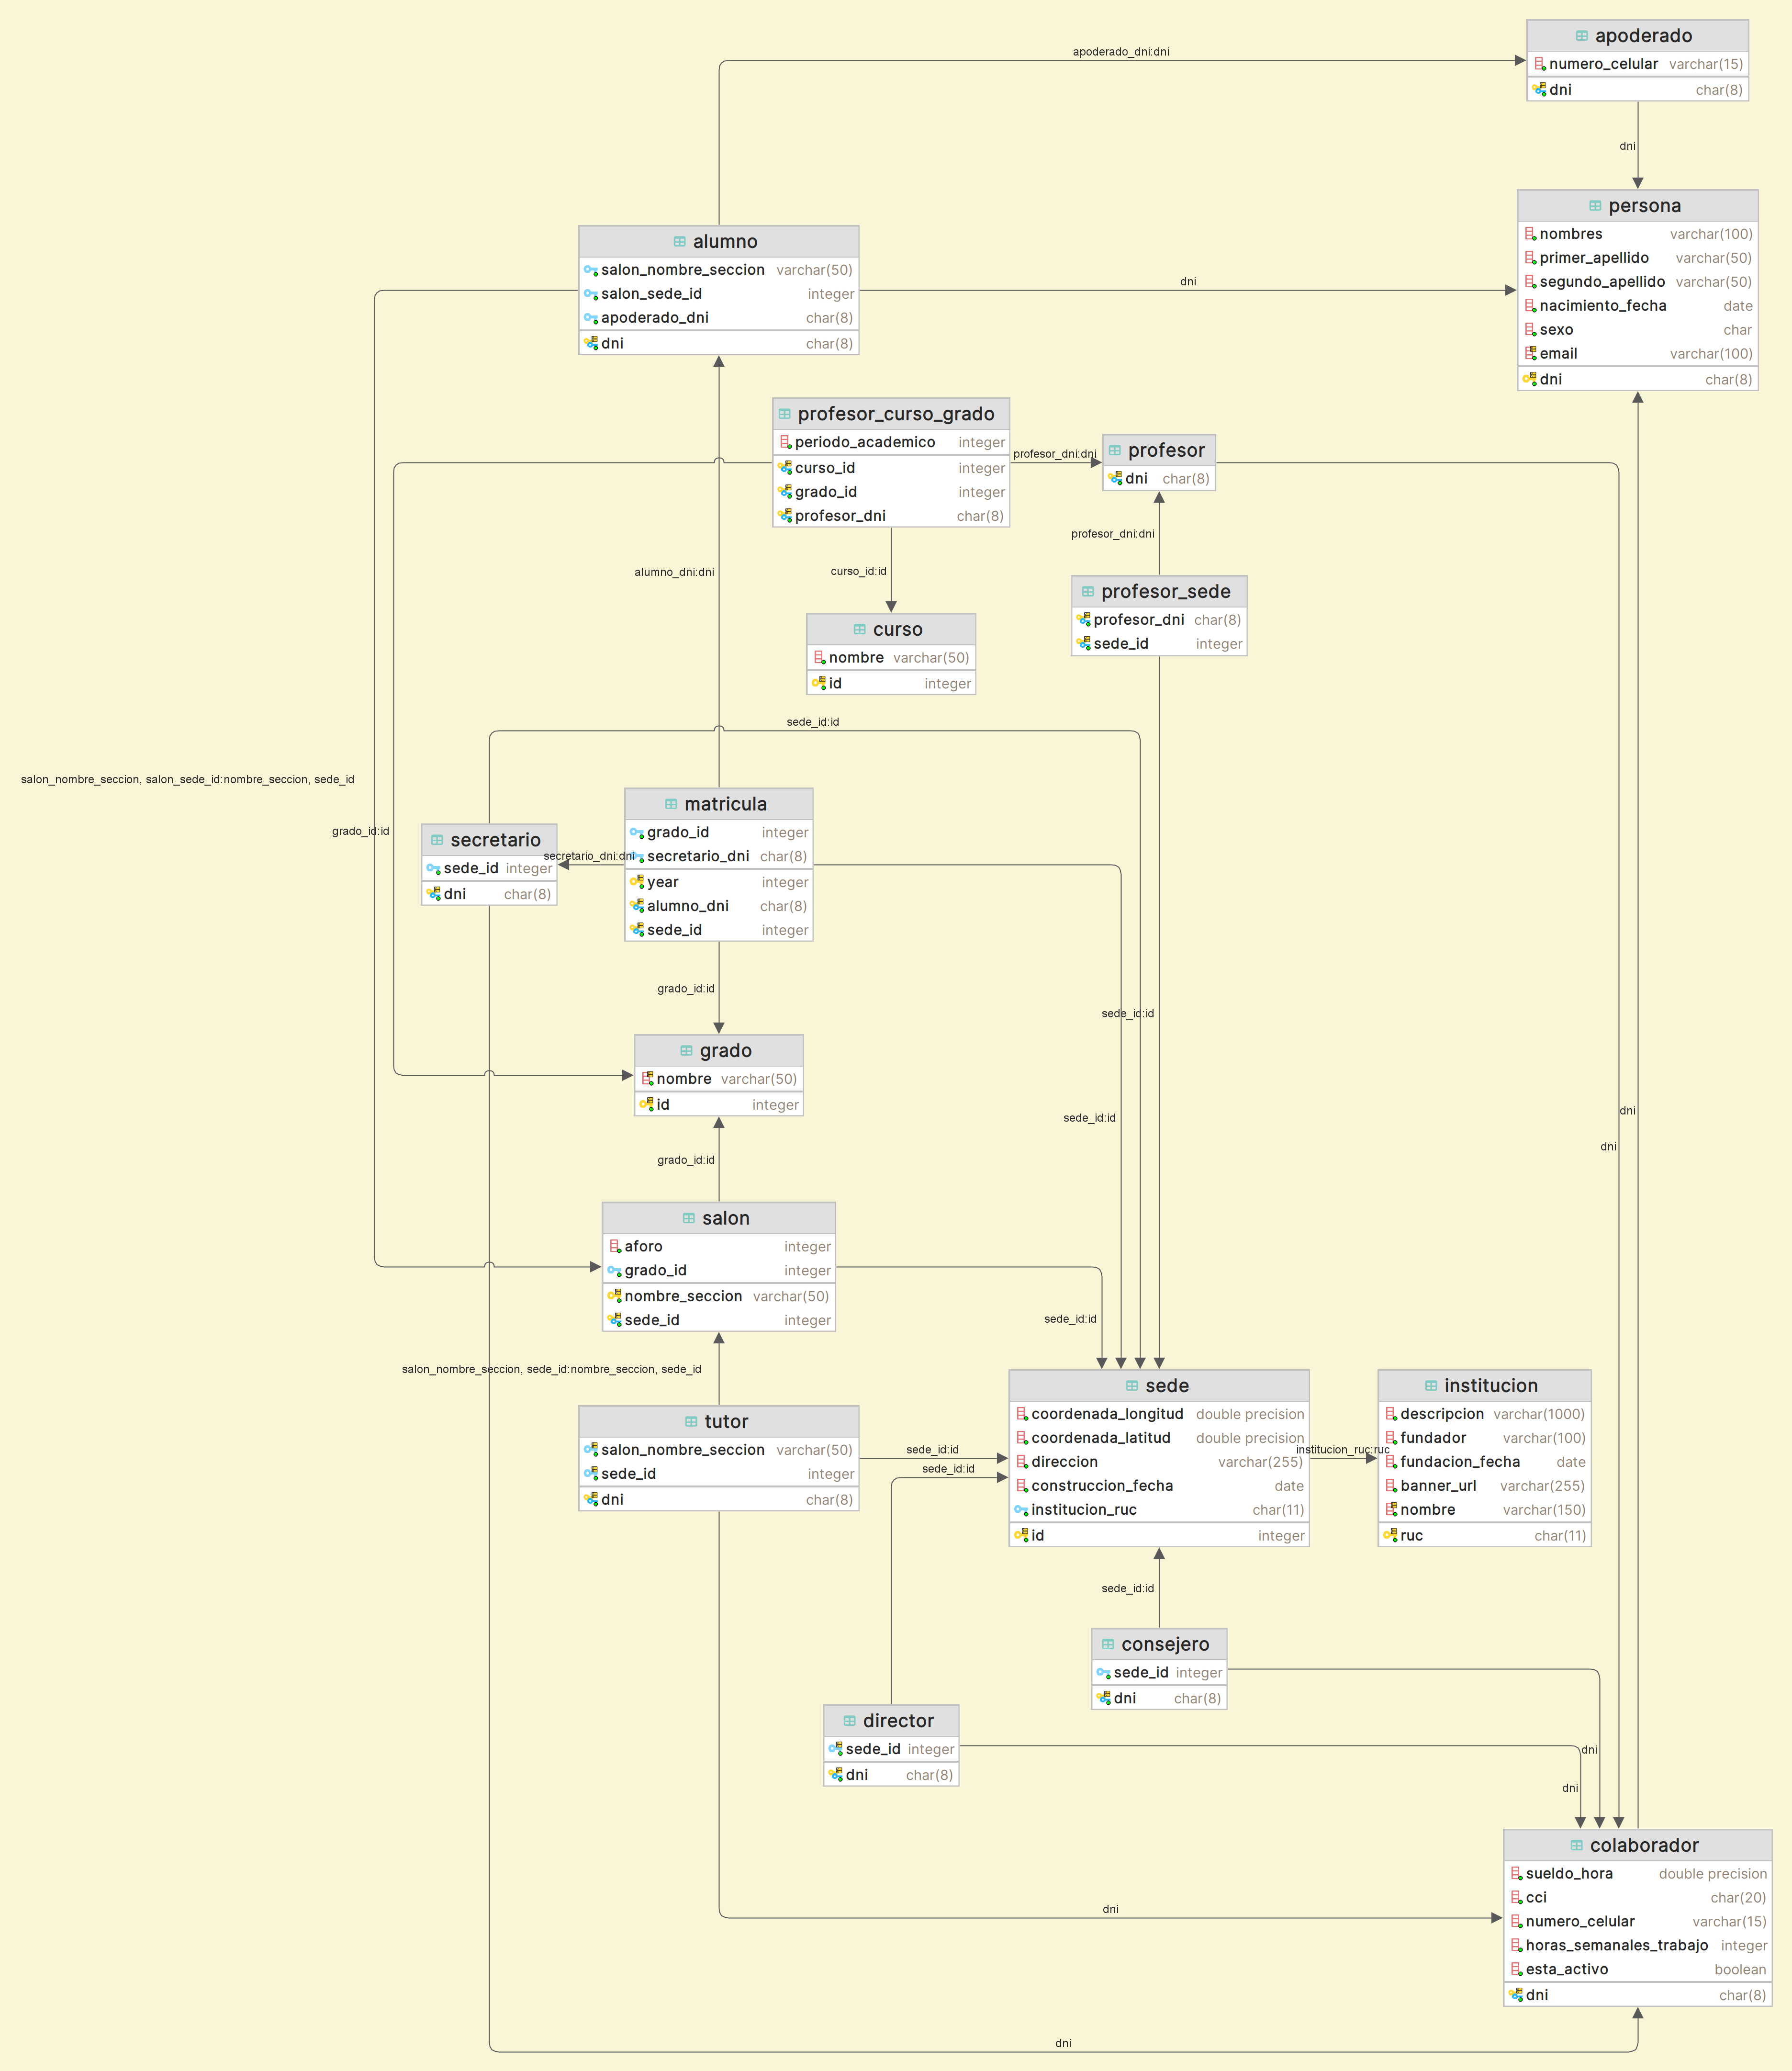
\includegraphics[width=\linewidth, height=0.75\textheight, keepaspectratio]{figures/modelo_fisico.png}
\end{center}
\subsection{Repositorios de GitHub}
\subsubsection{Repositorio del informe en LaTeX}{
    Este informe se ha realizado en LaTeX con el apoyo de GitHub, aprovechando sus herramientas de control de versiones y colaboración. La plataforma ha permitido documentar y gestionar cada etapa del proyecto con precisión. Para más detalles, acceda al repositorio en el siguiente enlace: \link{https://github.com/AlejandroEN/Database-I-Project-LaTex}{GitHub Repositorio}
}
\subsubsection{Repositorio del código en SQL}{
    Los contenidos del proyecto, incluidos el código SQL, el script de Python y los archivos CSV, se encuentran disponibles en otro repositorio de GitHub. Para más detalles, acceda al repositorio en el siguiente enlace: \link{https://github.com/AlejandroEN/Database-I-Project-Code}{GitHub Repositorio}
}
\subsection{Videos de experimentación}
\subsubsection{Consulta 1}
\begin{itemize}
    \item{\link{https://drive.google.com/file/d/1G6OM4pp-3xyTvn61H--6IS_XM8IY5r9Y/view?usp=drive_link}{Sin índices}}
    \item{\link{https://drive.google.com/file/d/1PIcvrEYvBltJCNQ3aT1Mw-3fVKul6ZF7/view?usp=drive_link}{Con índices por defecto}}
    \item{\link{https://drive.google.com/file/d/1Wq7pbkbU5-_EUVC_Qv5p91xKB4gqvnJg/view?usp=drive_link}{Con índices por defecto más índices personalizados}}
\end{itemize}
\subsubsection{Consulta 2}
\begin{itemize}
    \item{\link{https://drive.google.com/file/d/1MM1AwEC-DH_eJeznwzYpQitviGYUi5pc/view?usp=drive_link}{Sin índices}}
    \item{\link{https://drive.google.com/file/d/1YAjI4YJ9u9ZD81UBYiR_kSDgV5RDfJAJ/view?usp=drive_link}{Con índices por defecto}}
    \item{\link{https://drive.google.com/file/d/16mElSCN6Zkx0KVM7f2qu_xNKIKmU2ui0/view?usp=drive_link}{Con índices por defecto más índices personalizados}}
\end{itemize}
\subsubsection{Consulta 3}
\begin{itemize}
    \item{\link{https://drive.google.com/file/d/1F6jeoqpubWSvGTXQOKCm5BVJsAo3rnO6/view?usp=drive_link}{Sin índices}}
    \item{\link{https://drive.google.com/file/d/1AgnL8Z3CL18vB3-PS9tncTY-1QJVyCRd/view?usp=drive_link}{Con índices por defecto}}
    \item{\link{https://drive.google.com/file/d/1fa3fXZATm_HrQGIlS0w_1TQo3g1SDgrg/view?usp=drive_link}{Con índices por defecto más índices personalizados}}
\end{itemize}
\subsection{Pregunta extra}
¿Cuál sería la complejidad operacional si escalamos los datos por encima del millón?, realice una comparativa respecto a la cantidad de datos del párrafo anterior. ¿Es suficiente la arquitectura Cliente-Servidor para procesar millones de datos?

Para manejar eficientemente millones de datos, es fundamental optimizar la estructura de índices, particionar tablas, utilizar almacenamiento en caché y considerar bases de datos no relacionales (NoSQL). Sistemas como MongoDB y Cassandra son gestores de bases de datos no relacionales que facilitan la gestión de grandes volúmenes de datos y proporcionan flexibilidad en el modelado de datos. Por otro lado, la arquitectura Cliente-Servidor es suficiente si se optimiza adecuadamente, permite escalabilidad horizontal, implementa balanceadores de carga y mitiga cuellos de botella en la red, CPU y disco. Una arquitectura distribuida puede ser necesaria para gestionar eficientemente las operaciones a gran escala.
\printindex{}
\end{document}